\documentclass{beamer}

\usepackage{geometry}
\usepackage{graphicx}
%\usepackage{wrapfig}
\usepackage{amsmath}

%\useoutertheme{infolines}
\usetheme{Boadilla}
\usecolortheme{seahorse}
\setbeamertemplate{navigation symbols}{}
\title{Numbers}
\newcommand{\shorttitle}{64 Bit Intel Assembly Language}
\newcommand{\shortauthor}{\copyright 2011 Ray Seyfarth}
\author{Ray Seyfarth}
\begin{document}


\usefoottemplate{\vbox{
\tinycolouredline{structure!55}%
 {\color{white}{\textbf{\shorttitle}\hfill\textbf{\shortauthor}}}%
}}

\begin{frame}
    \titlepage
\end{frame}
\begin{frame}
\frametitle{Outline}
\tableofcontents
\end{frame}

\section{Binary numbers}

\begin{frame}
    \frametitle{Binary numbers}
\begin{itemize}
    \item Decimal place value system
\end{itemize}

\begin{align*}
15301201 &= 1*10^7 + 5*10^6 + 3*10^5 + 1^3 + 2*10^2 + 1 \\
         &= 10000000 + 5000000 + 300000 + 1000 + 200 + 1 \\
         &= 15301201
\end{align*}

\begin{itemize}
    \item Binary place value system
\end{itemize}

\begin{align*}
10101111 &= 2^7 + 2^5 + 2^3 + 2^2 + 2 + 1 \\
         &= 128 + 32 + 8 + 4 + 2 + 1 \\
         &= 175
\end{align*}

\end{frame}

\begin{frame}
    \frametitle{Bit numbering}
\begin{figure}[h!]
\centering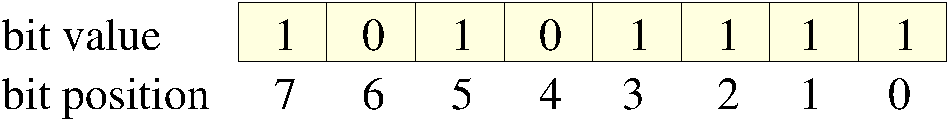
\includegraphics[width=0.8\textwidth]{175.pdf}
\end{figure}
\begin{itemize}
    \item The least significant bit of a byte is bit 0
    \item The most significant bit is bit 7
    \item In {\tt yasm} this number could be written as {\tt 10101111b}
\end{itemize}

\end{frame}

\begin{frame}
    \frametitle{Decimal to binary conversion}
            \begin{itemize}
                \item Convert 741 to binary
                \item Repeatedly divide by 2 and keep the remainders
            \end{itemize}

            \begin{tabular}{lrclcr}
            \quad\qquad & \multicolumn{3}{c}{division} & remainder & bits \\ \cline{2-6} 
            &741/2 &=& 370 & 1 & 1 \\
            &370/2 &=& 185 & 0 & 01 \\
            &185/2 &=& 92  & 1 & 101 \\
            &92/2  &=& 46  & 0 & 0101 \\
            &46/2  &=& 23  & 0 & 00101 \\
            &23/2  &=& 11  & 1 & 100101 \\
            &11/2  &=& 5   & 1 & 1100101 \\
            &5/2   &=& 2   & 1 & 11100101 \\
            &2/2   &=& 1   & 0 & 011100101 \\
            &1/2   &=& 0   & 1 & 1011100101 
            \end{tabular}
\end{frame}

\section{Hexadecimal numbers}
\begin{frame}
    \frametitle{Hexadecimal numbers}
    \begin{itemize}
        \item Base 16 numbers
        \item Use as ``digits'' 0-9 and A-F (or a-f)
        \item A=10, B=11, C=12, D=13, E=14, F=15
    \end{itemize}
\begin{align*}
{\tt 0x2b1a} &= 2*16^3 + 11*16^2 + 1*16 + 10 \\
             &= 2*4096 + 11*256 + 16 + 10 \\
             &= 8192 + 2816 + 16 + 10 \\
             &= 11034
\end{align*}
\end{frame}

\begin{frame}
    \frametitle{Why use hexadecimal?}
    \begin{itemize}
        \item Each hexadecimal digit or ``nibble'' is 4 bits
        \item {\tt 0x2b1a} = {\tt 0010 1011 0001 1010}
        \item {\tt 0x2b1a} = {\tt 0010101100011010b}
        \item Counting 32 bits for a binary pattern would be hard
        \item Hexadecimal is much easier
        \item {\tt 0xdeadbeef} = {\tt 11011110101011011011111011101111b}
    \end{itemize}
\end{frame}

\begin{frame}
    \frametitle{Converting decimal to hexadecimal}
            \begin{itemize}
                \item Convert 40007 to hexadecimal
                \item Repeatedly divide by 16 and keep the remainders
            \end{itemize}
\begin{tabular}{lrclcr}
\qquad\qquad & \multicolumn{3}{c}{division} & remainder & hex \\ \cline{2-6}
&40007/16 &=& 2500 & 7 & {\tt 7} \\
&2500/16  &=& 156  & 4 & {\tt 47} \\
&156/16   &=& 9    & 12 & {\tt c47} \\
&9/16     &=& 0    & 9  & {\tt 9c47} \\
\end{tabular}
\end{frame}

\section{Integers}

\begin{frame}
    \frametitle{Integers}
\begin{itemize}
    \item Integers can be 1, 2, 4 or 8 bytes long
    \item They can be signed or unsigned
\end{itemize}

\small
\begin{center}
\begin{tabular}{|c|c|c|c|c|}
\hline
Variety & Bits & Bytes & Minimum & Maximum \\
\hline
unsigned & 8   & 1     & 0       & 255 \\
\hline
signed & 8     & 1     & -128    & 127 \\
\hline
unsigned & 16  & 2     & 0       & 65535 \\
\hline
signed & 16    & 2     & -32768  & 32767 \\
\hline
unsigned & 32  & 4     & 0       & 4294967295 \\
\hline
signed & 32    & 4     & -2147483648    & 2147483647 \\
\hline
unsigned & 64  & 8     & 0       & 18446744073709551615 \\
\hline
signed & 64    & 8     & -9223372036854775808    & 9223372036854775807 \\
\hline
\end{tabular}
\end{center}
\end{frame}

\begin{frame}
    \frametitle{Negative integers}
    \begin{itemize}
        \item We use the highest-order bit as a sign bit
        \item 1 for a sign bit means a negative number
        \item If we stored -1 as 10000001b
        \item -1 + 1 would be 10000001b + 00000001b = 100000010b
        \item Then addition would yield -1 + 1 = -2
        \item There must be a better way to store negatives
        \item Hopefully, we can use the same circuitry for positives and negatives
    \end{itemize}

\end{frame}

\begin{frame}[fragile]
    \frametitle{Two's complement integers}
    \begin{itemize}
        \item To convert a number to its negative, use two's complement
        \item Flip all the bits
        \item Add 1
        \item Let's convert 1 to -1 with 8 bit numbers
    \end{itemize}
    \begin{verbatim}
             00000001 for the absolute value
             11111110 for the complement
             11111111 after adding 1 to the complement
        -1 = 11111111
    \end{verbatim}
    \begin{itemize}
        \item Two's complement negative numbers work for addition
    \end{itemize}
\end{frame}

\begin{frame}[fragile]
    \frametitle{More 8 bit signed integers}
    \begin{itemize}
        \item They form a cycle if you keep adding 1
    \end{itemize}
    \begin{verbatim}
        00000000 =    0
        00000001 =    1
        00000010 =    2
        ...
        01111111 =  127
        10000000 = -128
        10000001 = -127
        10000010 = -126
        ...
        11111110 =   -2
        11111111 =   -1
        00000000 =    0
    \end{verbatim}
\end{frame}

\begin{frame}[fragile]
\frametitle{Addition}
\small
\begin{itemize}
    \item Let's convert and add -29124 + 125
\end{itemize}
\begin{verbatim}
    29124  = 0111000111000100
    Negate = 1000111000111011
    Add 1  = 1000111000111100

      125  = 0000000001111101

    Now add  1000111000111100
             0000000001111101
             ----------------
             1000111010111001

    Negate   0111000101000110
    Add 1    0111000101000111
             28999

    So -29124 + 125 = -28999
\end{verbatim}
\end{frame}

\begin{frame}
\frametitle{Binary multiplication}
\begin{center}
\begin{tabular}{cr}
       & {\tt 1010101} \\
    *  & {\tt 10101} \\
\hline
       & {\tt 1010101} \\
       & {\tt 1010101\ \ } \\
       & {\tt 1010101\ \ \ \ } \\
\hline
       & {\tt 11011111001}
\end{tabular}
\end{center}
\end{frame}

\section{Floating point numbers}

\begin{frame}
    \frametitle{Floating point numbers}
    \begin{itemize}
        \item 32 bit, 64 bit and 80 bit numbers
        \item Stored in IEEE 754 format
    \end{itemize}

    \begin{center}
        \begin{tabular}{|l|c|c|c|c|c|}
        \hline
        Variety & Bits & Exponent & Exponent Bias & Fraction & Precision \\
        \hline
        float   &  32  & 8        &   127         & 23       & $\sim$7 digits \\
        \hline
        double  &  64  & 11       &  1023         & 52       & $\sim$16 digits \\
        \hline
        long double & 80 & 15     & 16383         & 64       & 19 digits \\
        \hline
        \end{tabular}
    \end{center}    
    \begin{itemize}
        \item Exponents are binary exponents
        \item An exponent field has the bias added
        \item A 32 bit exponent field of 128 means a binary exponent 1
        \item A 32 bit exponent field of 125 means a binary exponent -2
        \item 0.0 is stored as all bits equal to 0
        \item Exponent field 255 means ``Not a Number''
    \end{itemize}
\end{frame}

\begin{frame}
    \frametitle{Binary numbers with binary points}
\begin{align*}
    0.1_2   &= 2^{-1} \\
            &= 0.5 \\
    1.11_2  &= 1 + 2^{-1} + 2^{-2} \\
            &= 1 + 0.5 + 0.25 \\
            &= 1.75 \\
    1001.1001_2 &= 2^3 + 1 + 2^{-1} + 2^{-4} \\
              &= 8 + 1 + 0.5 + 0.0625 \\
              &= 9.5625 \\
    1.0010101 * 2^3 &= 1001.0101 \\
                  &= 2^3 + 1 + 2^{-2} + 2^{-4} \\
                    &= 8 + 1 + 0.25 + 0.0625 \\
                    &= 9.3125
\end{align*}
\end{frame}

\begin{frame}
    \frametitle{Implicit 1 bit}
\begin{figure}[h!]
\centering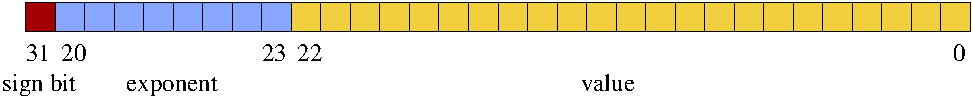
\includegraphics[width=0.95\textwidth]{float.pdf}
\end{figure}
    \begin{itemize}
        \item Normalized floats have exponent fields from 1 to 254
        \item For these floats there will be at least one 1 bit in the number
        \item IEEE 754 uses implicit 1 bits
        \item For non-zero floats, they can be written in ``scientific'' notation
        \begin{itemize}
            \item $1011.10101 = 1.01110101 * 2^3$
            \item The leading 1 bit is not stored
            \item The value (fraction) field is {\tt 01110101000000000000000}
        \end{itemize}
        \item So we have 23 bits of fraction with 1 implicit bit = 24 bits
        \item The sign bit is flipped to negate a float (1 means negative)
    \end{itemize}

\end{frame}

\begin{frame}[fragile]
    \frametitle{Floating point storage}
    \begin{itemize}
        \item Consider consider this listing by {\tt yasm}
    \end{itemize}

    \begin{verbatim}
    1                                 %line 1+1 fp.asm
    2                                 [section .data]
    3 00000000 00000000               zero dd 0.0
    4 00000004 0000803F               one dd 1.0
    5 00000008 000080BF               neg1 dd -1.0
    6 0000000C 0000E03F               a dd 1.75
    7 00000010 0000F542               b dd 122.5
    8 00000014 CDCC8C3F               d dd 1.1
    9 00000018 F9021550               e dd 10000000000.0
    \end{verbatim}
    \begin{itemize}
        \item The bytes are backwards
        \item 1.0 should be represented logically as {\tt 3F800000}
        \item 0 sign bit, 127 exponent field, 0 for the fraction field
    \end{itemize}
\end{frame}

\begin{frame}[fragile]
    \frametitle{Floating point storage (2)}
    \begin{verbatim}
    4 00000004 0000803F               one dd 1.0
    5 00000008 000080BF               neg1 dd -1.0
    6 0000000C 0000E03F               a dd 1.75
    7 00000010 0000F542               b dd 122.5
    \end{verbatim}
    \begin{itemize}
        \item All these have a lot of 0 bits in the fractions
        \item They are all exactly equal to a sum of a few powers of 2
        \item $1 = 2^0$
        \item $1.75 = 2^0 + 2^{-1} + 2^{-2}$
        \item $122.5 = 2^6+2^5+2^4+2^3+2^1+2^{-1}$
        \item -1.0 differs from 1.0 only in the sign bit
    \end{itemize}
\end{frame}

\begin{frame}[fragile]
    \frametitle{Floating point storage (3)}
    \begin{verbatim}
    8 00000014 CDCC8C3F               d dd 1.1
    \end{verbatim}
    \begin{itemize}
        \item 1.1 is a repeating binary number
        \item The number in ``proper'' order is {\tt 3F8CCCCD}
        \item The exponent field is 127, so the exponent is 1
        \item The number is $1.00011001100110011001101_2$
        \item It looks like $1.1 = 1.000\overline{1100}$
    \end{itemize}
\end{frame}

\section{Converting decimal numbers to floats}

\begin{frame}
    \frametitle{Converting decimal numbers to floats}
    \begin{itemize}
        \item Determine the sign bit and work with the absolute value
        \item Convert the whole part of the decimal number
        \item Convert the fraction
        \item Express in binary scientific notation
        \item Build the exponent field by adding 127 bias
        \item Drop the leading 1 to get the fraction field
        \item Example: convert -12.25
        \begin{itemize}
            \item Sign bit is 1
            \item Whole part is $12 = 1100_2$
            \item Fraction is $0.25 = 0.01$
            \item Scientific notation $12.25 = 1.10001_2 * 2^3$
        \end{itemize}
    \end{itemize}
        \begin{align*}
                -12.25 &= {\tt 1\ 10000010\ 10001000000000000000000} \\
                    &= {\tt 0xC1440000}
        \end{align*}
\end{frame}

\begin{frame}
    \frametitle{Converting decimal number to float (2)}
    \begin{itemize}
        \item The only non-obvious step is converting the fractional
            part to a binary fraction.
        \item Suppose you have a decimal number $x = .abcdefgh$
        \item Then if you multiple $x$ by 2, the only possible
            result is $2x < 1$ or $1 \le 2x < 2$
        \item If $2x < 1$, then $x < 0.5$, which means the first
            bit after the binary point is 0.
        \item If $2x \ge 1$, then $x \ge 0.5$, which means the first
            bit after the binary point is 1.
        \item So we set the first bit and work on the remaining
            fractional part of $2x$ to get the next bit.
        \item This process continues until we reach $x = 0$ or we
            have enough bits.
    \end{itemize}
\end{frame}

\begin{frame}
    \frametitle{Converting decimal number to float (3)}
    \begin{itemize}
        \item Let's convert $-121.6875$ to a binary number
        \item First the sign is 0
        \item $121 = 1111001_2$
        \item Now it's time to work on $.6875$
    \end{itemize}
    \begin{tabular}{ccccl}
        \quad\qquad &   Multiply& & Result & Binary \\
        &$.6875*2$ & $=$ & $1.375$ & $.1_2$ \\
        &$.375*2$ & $=$ & $0.75$ &   $.10_2$ \\
        &$.75*2$ & $=$ & $1.5$ &     $.101_2$ \\
        &$.5*2$ & $=$ & $1.0$ &      $.1011_2$ 
    \end{tabular}
    \begin{itemize}
        \item $-121.6875 = -1111001.1011_2$
        \item $-121.6875 = -1.1110011011_2 * 2^6$
        \item As a binary float {\tt 1 10000101 11100110110000000000000}
        \item Expressed in hexadecimal: {\tt 0xC2F36000}
    \end{itemize}
\end{frame}
        
\section{Floating point mathematics}

\begin{frame}
    \frametitle{Floating point addition}
    \begin{itemize}
        \item Let's add 41.275 and 0.315
        \item 41.275 = {\tt 101001.010001100110011010} in binary
        \item 0.325 = {\tt 0.0101000010100011110101110} in binary
        \item As with decimals, we align the numbers and add
    \end{itemize}
    \begin{tabular}{cll}
    \qquad\quad &     & {\tt 101001.010001100110011010} \\
       &  +   & {\tt \ \ \ \ \ 0.0101000010100011110101110}\\ \cline{2-3}
       &      & {\tt 101001.1001011100001010010101110}
    \end{tabular}
    \begin{itemize}
        \item There are 31 digits in the answer
        \item The answer must be rounded to 24 bits
        \item Rounding the last 7 bits means truncation in this case
        \item We get {\tt 0x42265c29} which is 41.59 (approximately)
    \end{itemize}

\end{frame}

\begin{frame}
    \frametitle{Floating point multiplication}
    \begin{itemize}
        \item Let's multiply 7.5 and 4.375
    \end{itemize}
    \begin{tabular}{ccrcr}
        \qquad\quad & &  7.5 & = & ${\tt 111.1}_2$ \\ 
        &* &  4.375 & = & ${\tt 100.011}_2$ \\ \cline{2-5}
        & &       &   & ${\tt 1111}_2$ \\
        & &       &   & ${\tt 11110}_2$ \\
        & &       &   & ${\tt 111100000}_2$ \\ \cline{2-5}
            &&       &   & ${\tt 100000.1101}_2$
    \end{tabular}
    \begin{itemize}
        \item Conversion to float format should be apparent by now
    \end{itemize}

\end{frame}

\end{document}
